\section[Decoupled model]{Solving a problem using a Decoupled Model}\label{tutorial-decoupled}
The process of solving a problem using \Dumux can be roughly divided into four parts: 
\begin{enumerate}
 \item The geometry of the problem and correspondingly a grid have to be defined.
 \item Material properties and constitutive relationships have to be defined.
 \item Boundary conditions as well as initial conditions have to be defined.
 \item A suitable model has to be chosen.
\end{enumerate}

In contrast to the last section, we now apply a decoupled solution procedure, a
so-called \textit{IMPET} (\textit{IM}plicit \textit{P}ressure \textit{E}xplicit 
\textit{T}ransport) algorithm. This means that the pressure equation is first 
solved using an implicit method. The resulting velocities are then used to solve
a transport equation explicitly.\\
In this tutorial, pure fluid phases are solved with a finite volume discretization
of both pressure- and transport step. Primary variables, according to default
settings of the model, are the pressure and the saturation of the wetting phase.

The problem which is solved in this tutorial is illustrated in figure 
\ref{tutorial-decoupled:problemfigure}. A rectangular domain with now flow 
boundaries on the top and at the bottom, which is initially saturated with oil, 
is considered. Water infiltrates from the left side into the domain. Gravity 
effects are neglected.

\begin{figure}[h]
\psfrag{x}{x}
\psfrag{y}{y}
\psfrag{no flow}{no flow}
\psfrag{water}{\textbf{water}}
\psfrag{oil}{\textcolor{white}{\textbf{oil}}}
\psfrag{p_w = 2 x 10^5 [Pa]}{$p_w = 2 \times 10^5$ [Pa]}
\psfrag{p_w_initial = 2 x 10^5 [Pa]}{\textcolor{white}{\textbf{$\mathbf{p_{w_{initial}} = 2 \times 10^5}$ [Pa]}}}
\psfrag{S_n = 0}{$S_w = 1$}
\psfrag{S_n_initial = 0}{\textcolor{white}{$\mathbf{S_{w_{initial}} = 0}$}}
\psfrag{q_w = 0 [kg/m^2s]}{$q_w = 0$ $\left[\frac{\textnormal{kg}}{\textnormal{m}^2 \textnormal{s}}\right]$}
\psfrag{q_n = -3 x 10^-4 [kg/m^2s]}{$q_n = -3 \times 10^-2$ $\left[\frac{\textnormal{kg}}{\textnormal{m}^2 \textnormal{s}}\right]$}
\centering
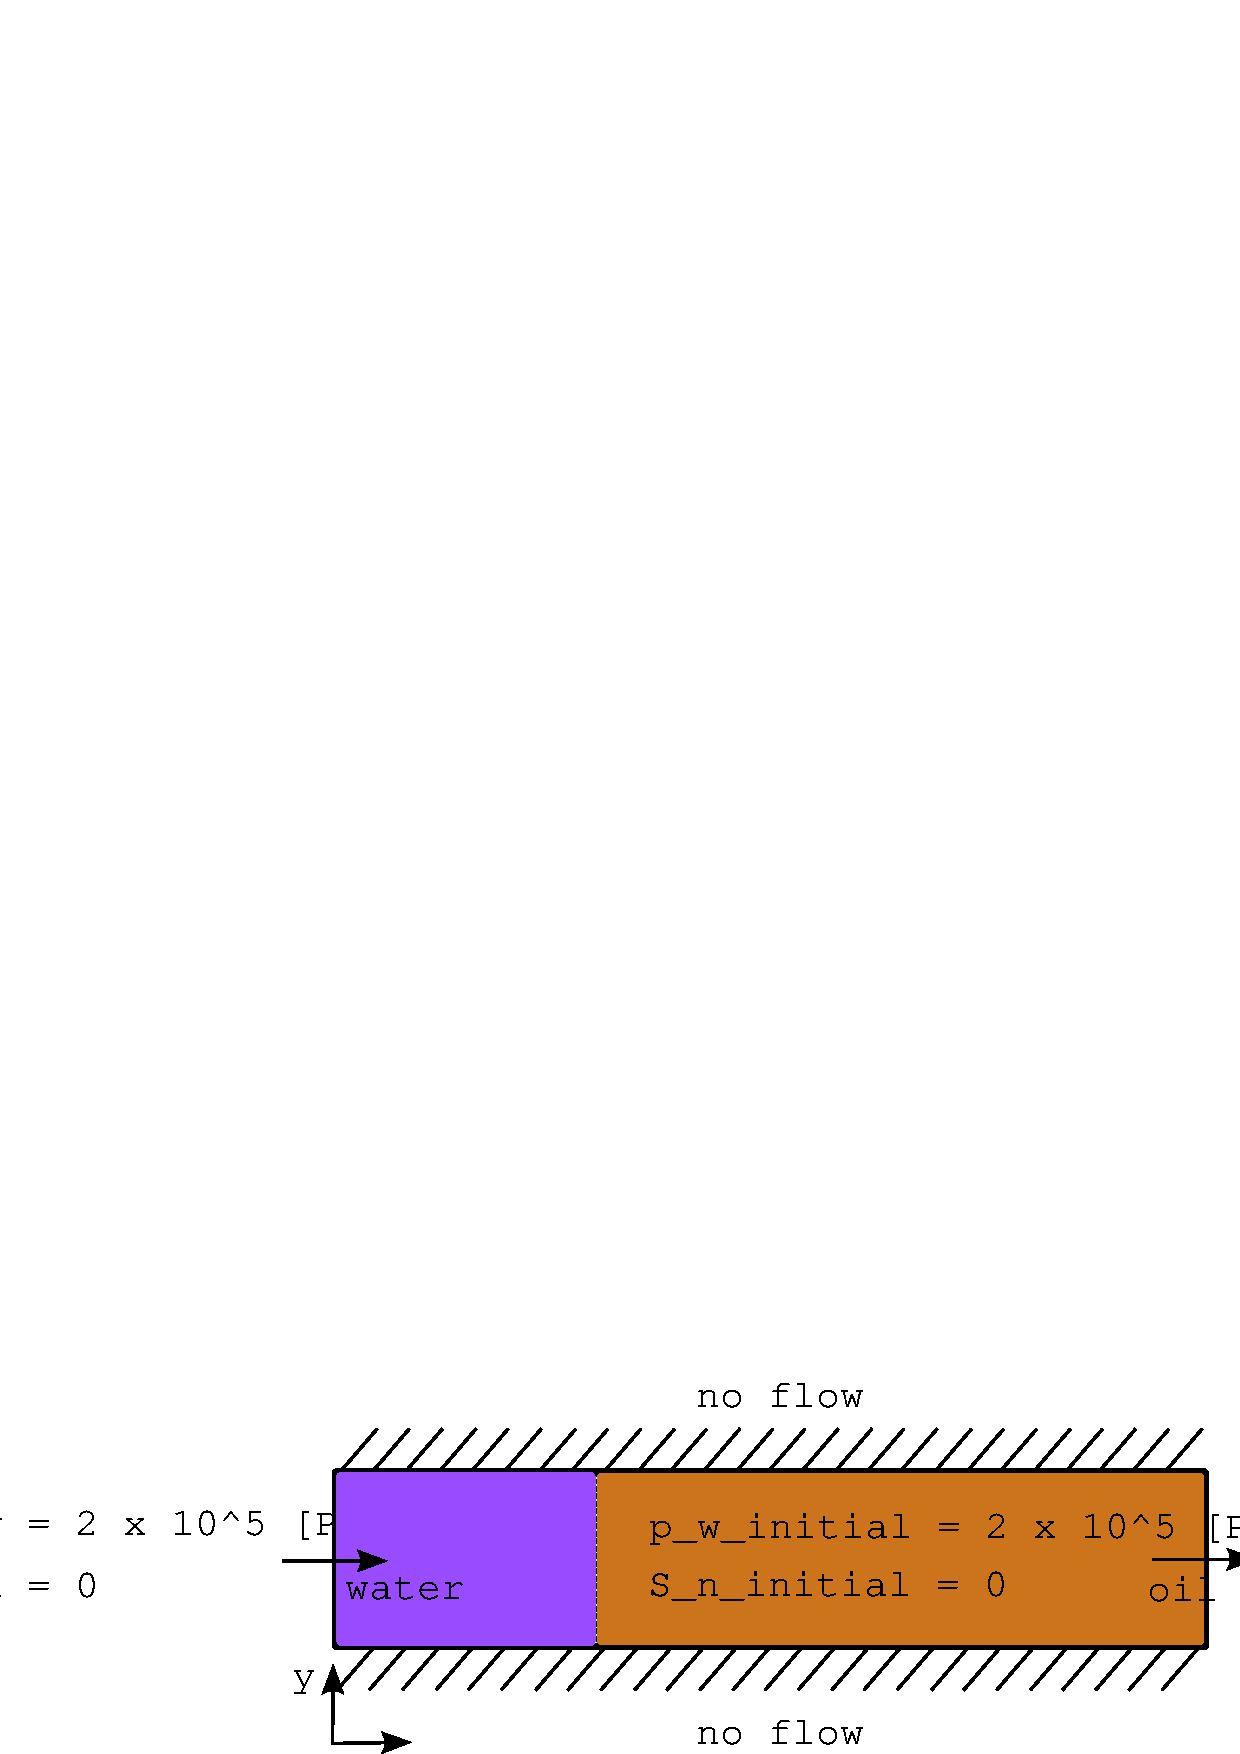
\includegraphics[width=0.9\linewidth,keepaspectratio]{EPS/tutorial-problemconfiguration}
\caption{Geometry of the tutorial problem with initial and boundary conditions.}\label{tutorial-decoupled:problemfigure}
\end{figure}

Listing \ref{tutorial-deoucpled:mainfile} shows how the main file, which has to be executed, has to be set up, if the problem described above is to be solved using a decoupled model. This main file can be found in the directory \texttt{/tutorial} of the stable part of \Dumux.

\begin{lst}[File tutorial/tutorial\_decoupled.cc]\label{tutorial-deoucpled:mainfile} \mbox{}
\lstinputlisting[basicstyle=\ttfamily\scriptsize,numbers=left, 
numberstyle=\tiny, numbersep=5pt, firstline=28]{../../tutorial/tutorial_decoupled.cc}
\end{lst}

First, from line \ref{tutorial-decoupled:include-begin} to line
\ref{tutorial-decoupled:include-end} the \Dune and \Dumux files containing
essential functions and classes are included.

At line \ref{tutorial-decoupled:set-type-tag} the type tag of the
problem which is going to be simulated is set. All other data types
can be retrieved by the \Dumux property system and only depend on this
single type tag. Retrieving them is done between line
\ref{tutorial-decoupled:retrieve-types-begin} and
\ref{tutorial-decoupled:retrieve-types-end}. For an introduction to the
property system, see section \ref{sec:propertysystem}.

The first thing which should be done at run time is to initialize the
message passing interface using \Dune's \texttt{MPIHelper} class. Line
\ref{tutorial-decoupled:init-mpi} is essential if the simulation is
intended to be run on more than one processor at the same time. Next,
the command line arguments are parsed starting at line
\ref{tutorial-decoupled:parse-args-begin} until line
\ref{tutorial-decoupled:parse-args-end}. In this case, we check weather and
at which time a previous run of the simulation should be restarted, and we
parse the time when the simulation ends. As the maximum time-step in the 
sequential model is strictly bound by a CFL-criterion, the first time-step
size is initialized with the simulation time.

After this, a grid is created on line \ref{tutorial-decoupled:create-grid} 
and the problem is instantiated with information about the grid
(via its leaf grid view) on line \ref{tutorial-decoupled:instantiate-problem}.
If demanded, on line \ref{tutorial-decoupled:mainRestart} a state written to
disk by a previous simulation run is restored on request by the user.
Finally, the time manager controlling the simulation run is instantiated 
with the start parameters in line \ref{tutorial-decoupled:initTimeManager}
and the simulation proceedure is started by the time manager at line
\ref{tutorial-decoupled:execute}.



\subsection{The problem class} \label{decoupled_problem}

When solving a problem using \Dumux, the most important file is the
so-called \textit{problem file} as shown in listing
\ref{tutorial-decoupled:problemfile} of
\texttt{tutorialproblem\_decoupled.hh}.

\begin{lst}[File tutorial/tutorialproblem\_decoupled.hh]\label{tutorial-decoupled:problemfile} \mbox{}
\lstinputlisting[basicstyle=\ttfamily\scriptsize,numbers=left,
numberstyle=\tiny, numbersep=5pt, firstline=28]{../../tutorial/tutorialproblem_decoupled.hh}
\end{lst}

First, both \Dune  grid handlers and the decoupled model of \Dumux 
have to be included. Then, a new type tag is created for the problem 
on line \ref{tutorial-decoupled:create-type-tag}.  In this case, the 
new type tag inherits all properties defined for the \texttt{DecoupledTwoP} 
type tag, which means that for this problem the two-phase decoupled approach
is chosen as discretization scheme (defined via the include in line 
\ref{tutorial-decoupled:parent-problem}). On line \ref{tutorial-decoupled:set-problem}, 
a problem class is attached to the new type tag, while the grid which
is going to be used is defined on line \ref{tutorial-decoupled:set-grid-type} --
in this case an \texttt{SGrid} is created.  Since in \Dune, there's no uniform
mechanism to allocate grids, the \texttt{Grid} property also contains
a static \texttt{create()} method which provides just that: From line 
\ref{tutorial-decoupled:grid-begin} to \ref{tutorial-decoupled:grid-end}, 
the geometry is defined and the grid is generated. The three variables of 
Type \texttt{Dune::FieldVector} define the lower left corner of the domain 
(\texttt{L}), the upper right corner of the domain (\texttt{H}) and the number 
of cells in $x$ and $y$ direction (\texttt{N}). The grid of type 
\texttt{Dune::SGrid} is then generated in line \ref{tutorial-decoupled:grid-end}. 
For more information about the \Dune grid interface, the different grid types 
that are supported and the generation of different grids it is referred to 
the \textit{Dune Grid Interface HOWTO} \cite{DUNE-HP}. 

Next, we select the material of the simulation: In case of a pure two-phase
model, each phase is a bulk fluid, and the complex (compositional) fluidsystems
do not need to be used. However, they can be used (see exercise 1 \ref{dec-ex1-fluidsystem}). 
Instead, we use a simplified fluidsystem container that provides classes 
for liquid and gas phases, line \ref{tutorial-decoupled:2p-system-start} to 
\ref{tutorial-decoupled:2p-system-end}. These are linked to the appropriate 
chemical species in line \ref{tutorial-decoupled:wettingPhase} and 
\ref{tutorial-decoupled:nonwettingPhase}. For all parameters that depend 
on space, such as the properties of the soil, the specific spatial parameters 
for the problem of interest are specified in line
\ref{tutorial-decoupled:set-spatialparameters}. 

Now we arrive at some model parameters of the applied two-phase decoupled 
model. Line \ref{tutorial-decoupled:velocityFormulation} defines that the 
wetting phase velocity rather than e.g. a total velocity is used for the 
transport system. As we regard capillary pressure, a capillary diffusive 
term is regarded, selected in line \ref{tutorial-decoupled:DiffusivePart}.
Line \ref{tutorial-decoupled:cfl} assigns the CFL-factor to be used in the
simulation run. The final property on line \ref{tutorial-decoupled:gravity} 
is optional and tells the model not to use gravity.

After all necessary information is written into the property system and 
its namespace is closed in line \ref{tutorial-decoupled:propertysystem-end},
the problem class is defined in line \ref{tutorial-decoupled:def-problem}. 
As its property, the problem class itsself is also derived from a parent, 
\texttt{IMPESProblem2P}. The class constructor (line 
\ref{tutorial-decoupled:constructor-problem}) is able to hold two vectors,
which is not needed in this tutorial.

Besides the definition of the boundary and initial conditions (discussed in 
subsection \label{decoupled-problem:boundary}), the problem class also contains
general information about the current simulation. First, the name used by
the \texttt{VTK-writer} to generate output is defined in the method of line
\ref{tutorial-decoupled:name}, and line \ref{tutorial-decoupled:restart} indicates
weather restart files are written. As decoupled schemes usually feature small 
timesteps, the method controlling the output in line \ref{tutorial-decoupled:output}
is very useful. The divisor of the modulo operation defines after how many timesteps
output should be written out -- the default ``1'' resembles output after each 
step.

The following methods all have in common that they may be dependent on space.
Hence, they all feature a common argument list:
\begin{itemize}
 \item \texttt{globalPos}: A vector holding the global Coordinates.
 \item \texttt{element} or \texttt{intersection}: Input for an iterator, that is 
    depending weather the parameter of the method is defined in an element, such as 
    initial values, or on an intersection, such as a boundary condition.
\end{itemize}
In the following, there are the methods for general parameters, source- or
sinkterms, boundary conditions (lines \ref{tutorial-decoupled:bctypePress} to
\ref{tutorial-decoupled:neumann}) and initial values for the transported
quantity in line \label{tutorial-decoupled:initSat}. For more information
on the functions, it is referred to the documentation in the code.

\subsection{The definition of the parameters that are dependent on space}\label{tutorial-decoupled:description-spatialParameters}

Listing \ref{tutorial-decoupled:spatialparametersfile} shows the file
\verb+tutorialspatialparameters_decoupled.hh+:

\begin{lst}[File tutorial/tutorialspatialparameters\_decoupled.hh]\label{tutorial-decoupled:spatialparametersfile} \mbox{}
\lstinputlisting[basicstyle=\ttfamily\scriptsize,numbers=left,
numberstyle=\tiny, numbersep=5pt, firstline=26]{../../tutorial/tutorialspatialparameters_decoupled.hh}
\end{lst}
As this file only slightly differs from the coupled version, it is referred to 
chapter \ref{tutorial-coupled:description-spatialParameters} for explanations.
However, as a standard Finite-Volume--scheme is used, in contrast to the box-method
in the coupled case, the argument list here is the same as for the problem 
functions:
\begin{itemize}
 \item \texttt{globalPos}: A vector holding the global Coordinates.
 \item \texttt{element}: Input for an element iterator, providing access
	to the current element of interest.
\end{itemize}

\subsection{Exercise}
\label{tutorial-deoucpled:exercises}
The following exercises will give you the opportunity to learn how you can change 
soil parameters, boundary conditions and fluid properties in \Dumux and to play along 
with the decoupled modelling framework.

\subsubsection{Exercise 1}
\renewcommand{\labelenumi}{\alph{enumi})}
For Exercise 1 you only have to make some small changes in the tutorial files.
\begin{enumerate}
\item \textbf{Altering output}
To get an impression what the results should look like you can first run the original version of the decoupled tutorial model by typing  \texttt{./tutorial\_decoupled 1e5}. The number behind the simulation name defines the timespan of the simulation run in seconds. For the visualisation with paraview please refer to \ref{quick-start-guide}.\\
As you can see, the simulation creates roughly 150 output files. To reduce these to perform longer simulations, change the method responsible for output (line \ref{tutorial-decoupled:output} in the file \texttt{tutorialproblem\_decoupled}) to write an output only every 20 timesteps by changeing the divisor. Compile the main file by typing \texttt{make tutorial\_decoupled} and run the model. Now, run the simulation for 5e5 seconds.

\item \textbf{Changing the Model Domain and the Boundary Conditions} \\
Change the size of the model domain so that you get a rectangle
with edge lengths of x = 300 m \\  and y = 300 m and with discretisation lengths of  $\Delta \text{x} = 20$ m and $\Delta \text{y} = 10$ m. \\
Change the boundary conditions in the file \texttt{tutorialproblem\_decoupled.hh} so that water enters from the bottom and oil flows out at the top boundary. The right and the left boundary should be closed for water and oil fluxes.  \\

\item \textbf{Changing Fluids} \\
Now you can change the fluids. Use DNAPL instead of Oil and Brine instead of Water. To do that you have to select different components via the property system in the problem file:
\begin{enumerate}
 \item Brine: The class \texttt{Dumux::Brine} acts as a adapter to the fluid system that alters a pure water class by adding some salt. Hence, the class \texttt{Dumux::Brine} uses a pure water class, such as \texttt{Dumux::H2O}, as a second template argument after the data type \texttt{<Scalar>} as a template argument (be aware to use the complete water class with its own template parameter).
 \item DNAPL: A standard set of chemical substances, such as Oil and Brinde, is already included (via a list of \texttt{\#include ..} commandos) and hence easy accessible by default. This is not the case for the class \texttt{Dumux::SimpleDNAPL}, however, which is located in the folder \texttt{dumux/material/components/}. Try to include the file as well as select the component via the property system.
\end{enumerate}
If you want to take a closer look how the fluid classes are defined and which substances are already available please browse through the files in the directory
\texttt{/dumux/material/components}.

\item \textbf{Use the \Dumux fluid system}\label{dec-ex1-fluidsystem} \\
As you have experienced in the coupled tutorial (chapter \ref{tutorial-decoupled}), \Dumux usually organises fluid mixtures via a \texttt{fluidsystem}. This is also possible for the decoupled models: Uncomment, as we want to reuse it later on, the lines \ref{tutorial-decoupled:2p-system-start} to \ref{tutorial-decoupled:2p-system-end} in the problem file. If you use eclipse, this can easily be done by pressing \textit{str + shift + 7}, the same shortcut works to cancel the comment later on.\\
Now include the file \texttt{fluidsystems/h2o\_n2\_system.hh} in the material folder, and set a property \texttt{FluidSystem} with the appropriate type, \texttt{Dumux::H2O\_N2\_System<TypeTag>}. However, the complicated fluidsystem uses tabularized fluid data, which need to be initialized in the constructor body of the current problem by adding \texttt{GET\_PROP\_TYPE(TypeTag, PTAG(FluidSystem))::init();}, hence using the initialization function of the applied fluidsystem. As an alternative, use a simpler version of water, e.g. \texttt{Dumux::SimpleH2O}, and apply it for the property \texttt{Components} with type \texttt{H2O}. The density of the gas is magnitudes smaller than that of oil, so please decrease the injection rate to $q_n = -3 \times 10^-4$ $\left[\frac{\textnormal{kg}}{\textnormal{m}^2 \textnormal{s}}\right]$. Also reduce the simultation duration to 2e4 seconds.\\
Please reverse the changes of this example, as we still use bulk phases and hence do not need such an extensive fluid system.
 
\item \textbf{Heterogeneities}  \\
Set up a model domain with the soil properties given in Figure \ref{tutorial-deoucpled:exercise1_d}. Adjust the boundary conditions so that water is again flowing from left to right.
\begin{figure}[h]
\psfrag{K1 =}{K $= 10^{-8}\text{ m}^2$}
\psfrag{phi1 =}{$\phi = 0.15$}
\psfrag{K2 =}{\textcolor{white}{K $= 10^{-9}\text{ m}^2$}}
\psfrag{phi2 =}{\textcolor{white}{$\phi = 0.3$}}
\psfrag{600 m}{600 m}
\psfrag{300 m}{300 m}
\centering
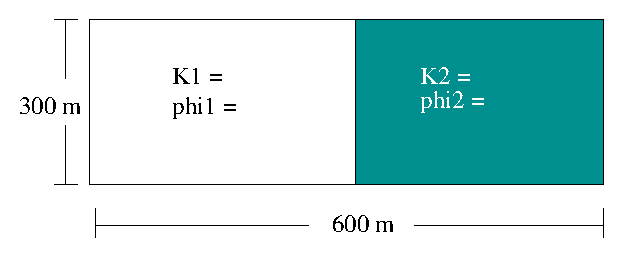
\includegraphics[width=0.5\linewidth,keepaspectratio]{EPS/exercise1_c.eps}
\caption{Exercise 1d: Set-up of a model domain a heterogeneity. $\Delta \text{x} = 20$ m $\Delta \text{y} = 20$ m.}\label{tutorial-deoucpled:exercise1_d}
\end{figure}
When does the front cross the material border? In paraview, the option \textit{View} $\rightarrow$ \textit{Animation View} is nice to get a rough feeling of the timestep sizes.
\end{enumerate}

\subsubsection{Exercise 2}
For this exercise you should create a new proplem file analogous to
the file \texttt{tutorialproblem\_decoupled.hh} (e.g. with the name 
\texttt{ex2\_tutorialproblem\_decoupled.hh} and new spatial parameters 
just like \texttt{tutorialspatialparameters\_decoupled.hh}. These files need to
be included in the file \texttt{tutorial\_decoupled.cc}. 

The new files should contain the definition of a new classes with 
names that relate to the file name, such as \texttt{Ex2TutorialProblemDecoupled}. 
Make sure that you also adjust the guardian
macros in lines \ref{tutorial-decoupled:guardian1} and \ref{tutorial-decoupled:guardian2}
 in the header files (e.g. change \\
\texttt{DUMUX\_TUTORIALPROBLEM\_DECOUPLED\_HH} to
\texttt{DUMUX\_EX2\_TUTORIALPROBLEM\_DECOUPLED\_HH}).  Besides also adjusting the guardian macros, 
the new problem file should define and use a new type tag for the problem as well as a new problem class
e.g. \texttt{Ex2TutorialProblemDecoupled}. Make sure you assign your newly defined spatial 
parameter class to the \texttt{SpatialParameters} property for the new 
type tag. 

After this, change the \texttt{create()} method of the \texttt{Grid}
property so that it matches the domain described
by figure \ref{tutorial-decoupled:ex2_Domain}. Adapt the problem class
so that the boundary conditions are consistent with figure
\ref{tutorial-decoupled:ex2_BC}. Initially the domain is fully saturated
with water and the pressure is $p_w = 2 \times 10^5 \text{Pa}$ . Oil
infiltrates from the left side. Create a grid with $20$ cells in
$x$-direction and $10$ cells in $y$-direction. The simulation time
should be set to $2e4 \text{s}$.

Now include your new problem file in the main file and replace the
\texttt{TutorialProblemDecoupled} type tag by the one you've created and
compile the program.


\begin{figure}[h]
\psfrag{K1}{K $= 10^{-7}\text{ m}^2$}
\psfrag{phi1}{$\phi = 0.2$}
\psfrag{Lin}{Brooks Corey Law} 
\psfrag{Lin2}{$\lambda = 1.8$, $p_b = 100$}
\psfrag{K2}{K $= 10^{-9}\text{ m}^2$}
\psfrag{phi2}{$\phi = 0.15$}
\psfrag{BC1}{Brooks Corey Law} 
\psfrag{BC2}{$\lambda = 2$, $p_b = 500$}
\psfrag{H1y}{50 m}
\psfrag{H2y}{15 m}
\psfrag{H3y}{20 m}
\psfrag{L1x}{100 m}
\psfrag{L2x}{50 m}
\psfrag{L3x}{25 m}
\centering
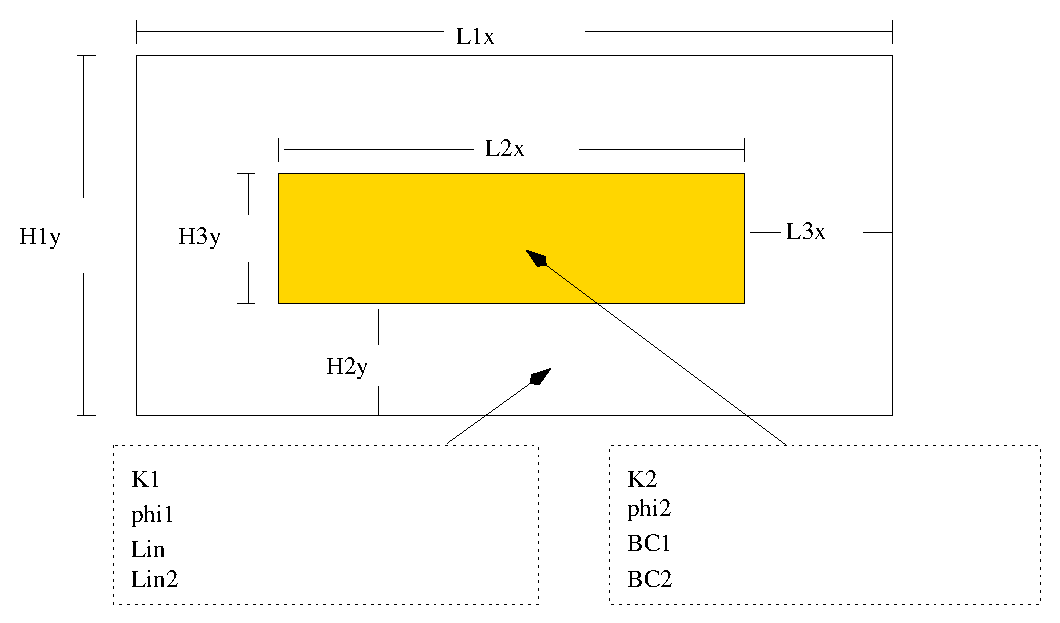
\includegraphics[width=0.8\linewidth,keepaspectratio]{EPS/Ex2_Domain.eps}
\caption{Set-up of the model domain and the soil parameters}\label{tutorial-decoupled:ex2_Domain}
\end{figure}

\begin{figure}[h]
\psfrag{pw}{$p_w = 2 \times 10^5$ [\text{Pa}]}
\psfrag{S}{$S_w = 0.0$}
\psfrag{qw}{$q_w = 3 \times 10^{-4}$ [kg/$\text{m}^2$s]}
\psfrag{qo}{$q_n = 0.0$ [kg/$\text{m}^2$s]}
\psfrag{no flow}{no flow}
\centering
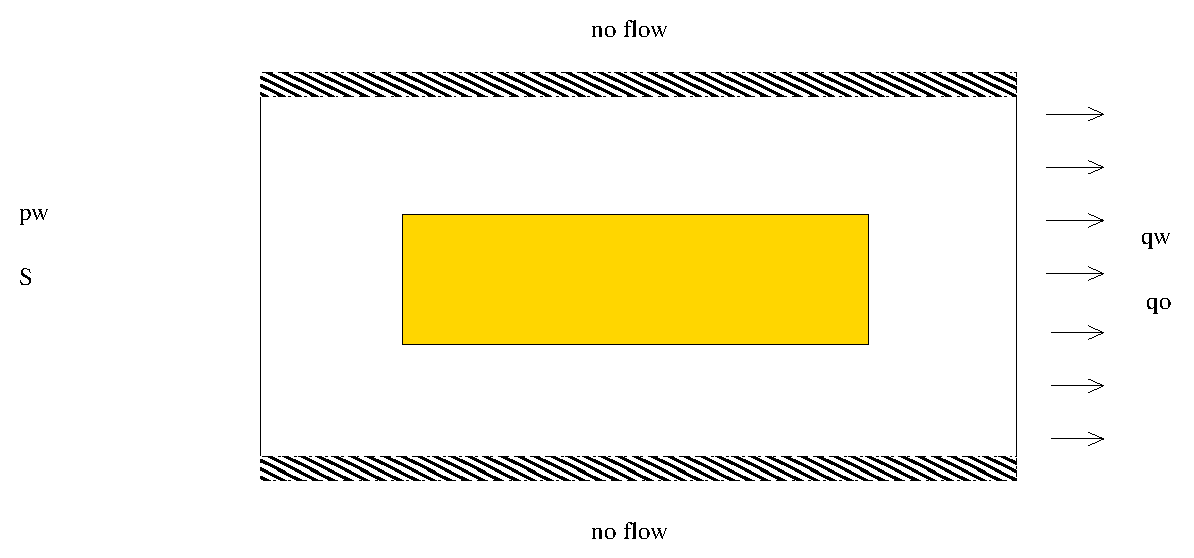
\includegraphics[width=0.8\linewidth,keepaspectratio]{EPS/Ex2_Boundary.eps}
\caption{Boundary Conditions}\label{tutorial-decoupled:ex2_BC}
\end{figure}

\begin{itemize}
 \item What happens if you increase the resolution of the grid? Hint: Paraview can visualize the timesteps via the ``Animation View'' (to be enabled unter the button \textit{View}).
 \item Set the CFL-factor to 1 and investigate the saturation: Is the value range reasonable?
 \item Further increase the CFL-factor to 2 and investigate the saturation.
\end{itemize}


\subsubsection{Exercise 3}
Create a new file for benzene called \texttt{benzene.hh} and implement
a new fluid system. (You may get a hint by looking at existing fluid 
systems in the directory \verb+/dumux/material/fluidsystems+.)

Use benzene as a new fluid and run the model of Exercise 2 with water
and benzene. Benzene has a density of $889.51 \, \text{kg} / \text{m}^3$
and a viscosity of $0.00112 \, \text{Pa} \; \text{s}$. 

%%% Local Variables: 
%%% mode: latex
%%% TeX-master: "dumux-handbook"
%%% End: 
